\documentclass[11pt]{beamer}
\usetheme{Boadilla}
\usepackage[utf8]{inputenc}
\usepackage{amsmath}
\usepackage{amsfonts}
\usepackage{amssymb}
%\author{}
\title{Hybrid model}
%\setbeamercovered{transparent}
%\setbeamertemplate{navigation symbols}{}
%\logo{}
%\institute{}
%\date{}
%\subject{}
\begin{document}

\begin{frame}
\titlepage
\end{frame}

%\begin{frame}
%\tableofcontents
%\end{frame}

\begin{frame}{"Final" model}
\begin{eqnarray}
\nonumber
\frac{p}{E}\cdot \partial f = {\color{red} C^{2\leftrightarrow 2, 2\leftrightarrow 3}_{\textrm{pQCD}}[f]} + {\color{blue} C_{\textrm{Diff}}[f]}
\end{eqnarray}
{\color{red} A "basic" pQCD model.}
\begin{itemize}
\item "Basic": no magic tuning, no K-factor, $\alpha_s$ under control.
\item Only uncertainty comes from the scale at which $\alpha_s$ is evaluated.
\end{itemize}
{\color{blue} A diffusion component parametrizes what is missing from pQCD.}
\begin{itemize}
\item $\hat{q}(T, E)$ can be completely parametric. Problem: $\hat{q}_c$, $\hat{q}_b$?
\item Or, guided by a simple parametric model. Fit a single set of parameter for both $c$ and $b$.
\end{itemize}
\end{frame}

\begin{frame}{The pQCD component}
Elastic process: intermediate propagators are all screened by Debye mass.
\begin{eqnarray}
\nonumber
\frac{1}{s}, \frac{1}{t}, \frac{1}{u} \rightarrow \frac{1}{s+m_D^2}, \frac{1}{t-m_D^2}, \frac{1}{u+m_D^2}
\end{eqnarray}
Debye mass: simplest leading order result.
\begin{eqnarray}
\nonumber
m_D^2 = \frac{4\pi}{3}\left(Nc+\frac{N_f}{2}\right)\alpha_s T^2
\end{eqnarray}
Inelastic process: Gunion-Bertsch matrix-element, with interference between subsequent radiation/absorption.
\begin{eqnarray}
\nonumber
\frac{dP}{dq dk^3 dt} = \frac{dP_{GB}}{dq dk^3 dt} \left(1-\cos\left(\frac{\Delta t}{\tau_k}\right)\right)
\end{eqnarray}
\end{frame}

\begin{frame}{The pQCD component: control running coupling}
Running coupling is difficult for multi-scale problem:
$T$, $Q^2$, $k_\perp^2$.
\begin{itemize}
\item For probe-medium interaction:
\begin{eqnarray}
\nonumber
|M_{2\leftrightarrow 2}|^2 &\propto& \alpha_s^2(Q^2, T) \\
\nonumber
|M_{2\leftrightarrow 2}|^2 &\propto& \alpha_s^2(Q^2, T) \alpha_s(k_\perp^2, T)
\end{eqnarray}
\item In medium, no process slower than $t\sim 1/T$ can exist alone, since the thermal collision rate $\propto T$. So $\alpha_s$ scale has a lower limit of $O(T)$,
\begin{eqnarray}
\nonumber
\alpha_s(\mu) = \alpha_s(\mu = \max\{Q, \mu_0 T\}),\\
\nonumber
\alpha_s(\mu) = \alpha_s(\mu = \max\{k_\perp, \mu_0 T\}).
\end{eqnarray}
Coupling constant must be smaller than $\alpha_s(\mu_0 T)$, $\mu_0$ is uncertain ($\pi T$, $2\pi T$, or any number within a reasonable range).
\end{itemize}
\end{frame}

\begin{frame}{pQCD: average $\alpha_s(\mu)$}
The averaged coupling constant of elastic processes. The uncertainty of $\mu_0$ leads to large uncertainty in scattering rates (like a K-factor but with $E, T$-dependence).
\begin{center}
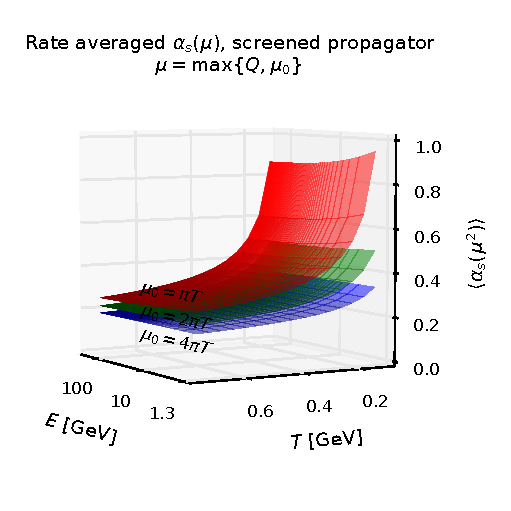
\includegraphics[width=0.5\textwidth]{fig/charm-plot/avg_alphas.pdf}
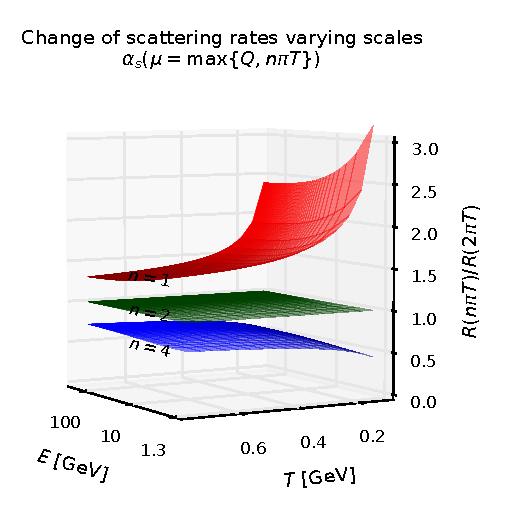
\includegraphics[width=0.5\textwidth]{fig/charm-plot/Rscale.pdf}
\end{center}
\end{frame}

\begin{frame}{pQCD: thermalization time of charm vs bottom, $\mu = 2\pi T$}
To see the approach to thermalization of an ensemble of particles $\{E_i\}$,
\begin{eqnarray}
\nonumber
\Delta S = \left\langle \ln(f_0(E_i)) \right\rangle_i - \int f_0(E) \ln(f_0(E)) dE
\end{eqnarray}
\begin{center}
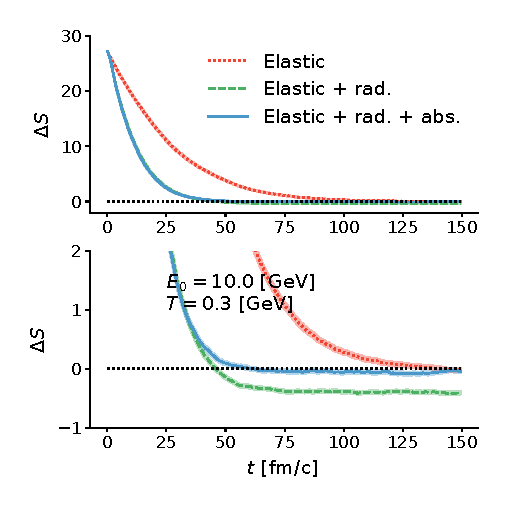
\includegraphics[width=0.5\textwidth]{fig/charm-plot/thermalization.pdf}
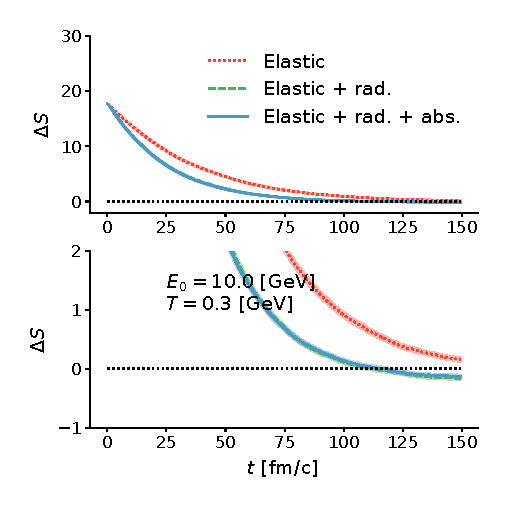
\includegraphics[width=0.5\textwidth]{fig/bottom-plot/thermalization.pdf}
\end{center}
\end{frame}

\begin{frame}{pQCD: $\Delta E$-$E$ in box, charm vs bottom, $\mu = 2\pi T$}
\begin{overprint}
\onslide<1> 
Charm: radiative E-loss dominates at large energy.
\onslide<2> 
Bottom: similar elastic E-loss as charm, but much less radiative E-loss.
\end{overprint}
\begin{overprint}
\onslide<1> 
\begin{center}
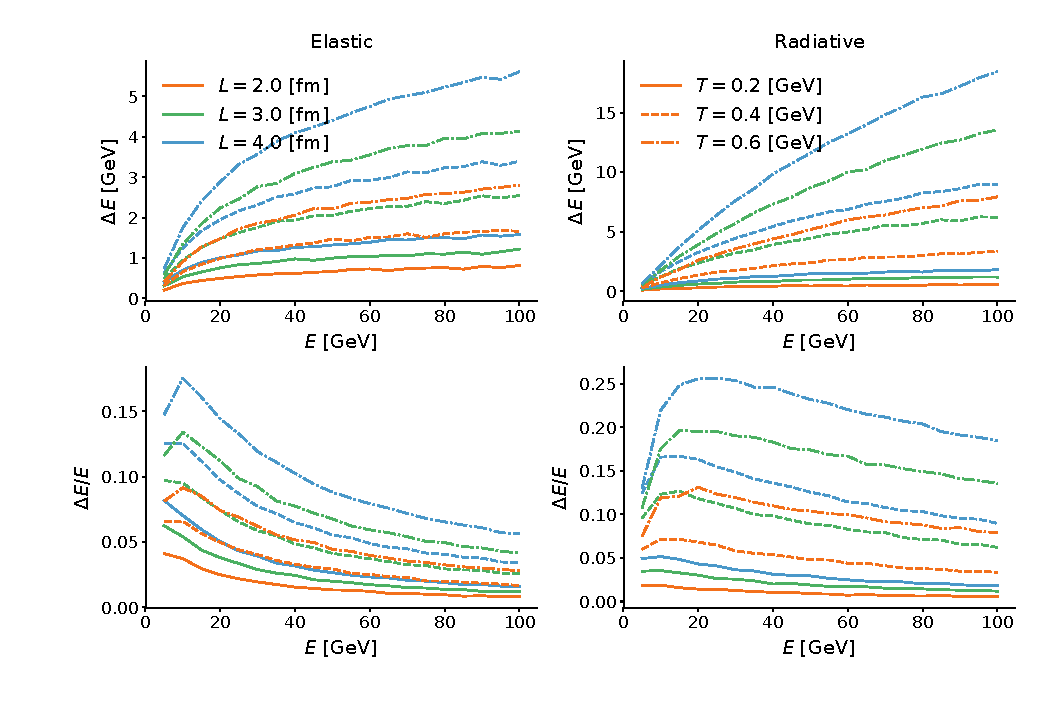
\includegraphics[width=\textwidth]{fig/charm-plot/E_Eloss.pdf}
\end{center}
\onslide<2> 
\begin{center}
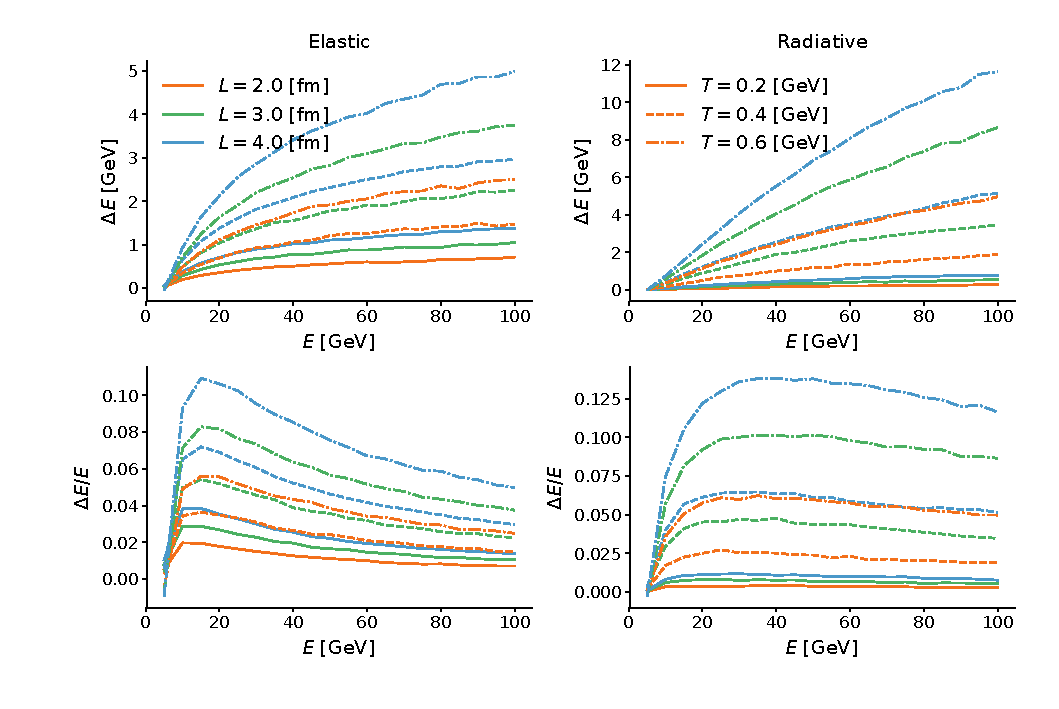
\includegraphics[width=\textwidth]{fig/bottom-plot/E_Eloss.pdf}
\end{center}
\end{overprint}
\end{frame}

\begin{frame}{pQCD: $\Delta E$-$L$ in box, charm vs bottom, $\mu = 2\pi T$}
\begin{overprint}
\onslide<1> 
Charm: non-linear $\Delta E-L$ behavior at small length.
\onslide<2> 
Bottom: again similar elastic E-loss, but less radiative E-loss.
\end{overprint}

\begin{overprint}
\onslide<1> 
\begin{center}
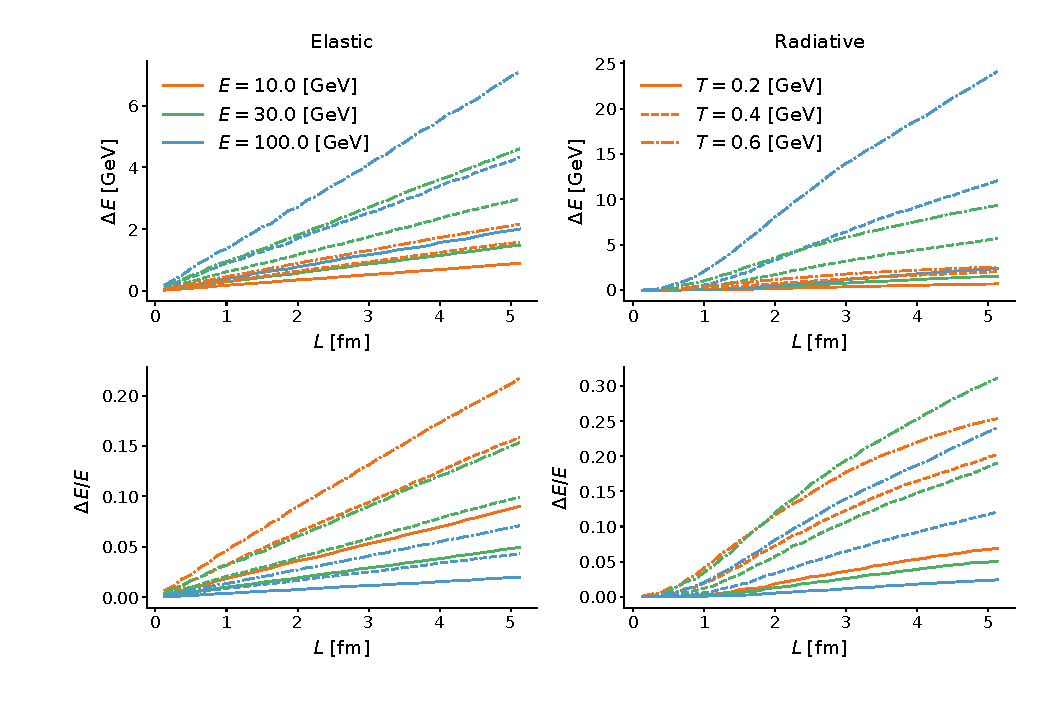
\includegraphics[width=\textwidth]{fig/charm-plot/L_Eloss.pdf}
\end{center}
\onslide<2> 
\begin{center}
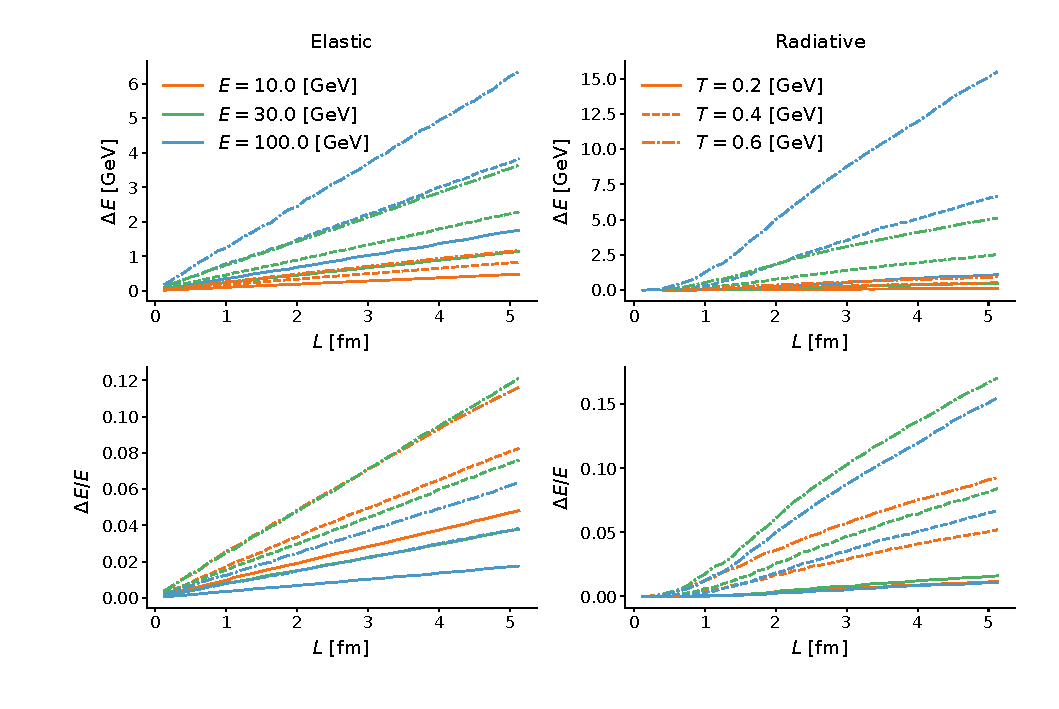
\includegraphics[width=\textwidth]{fig/bottom-plot/L_Eloss.pdf}
\end{center}
\end{overprint}
\end{frame}

\begin{frame}{pQCD: relative importance of $\Delta E_{\textrm{el}}$ vs $\Delta E_{\textrm{rad}}$, $\mu = 2\pi T$}
\begin{overprint}
\onslide<1> 
Charm: \\
It looks $\Delta E_{\textrm{rad}}$) always contributes $>50\%$ for large path length.\\
$\Delta E_{\textrm{el}}$ only dominates at small path length (where LPM is important).
\onslide<2> 
Bottom: $\Delta E_{\textrm{rad}}$ not important at very low energy ($E<5 GeV$)
\end{overprint}

\begin{overprint}
\onslide<1> 
\begin{center}
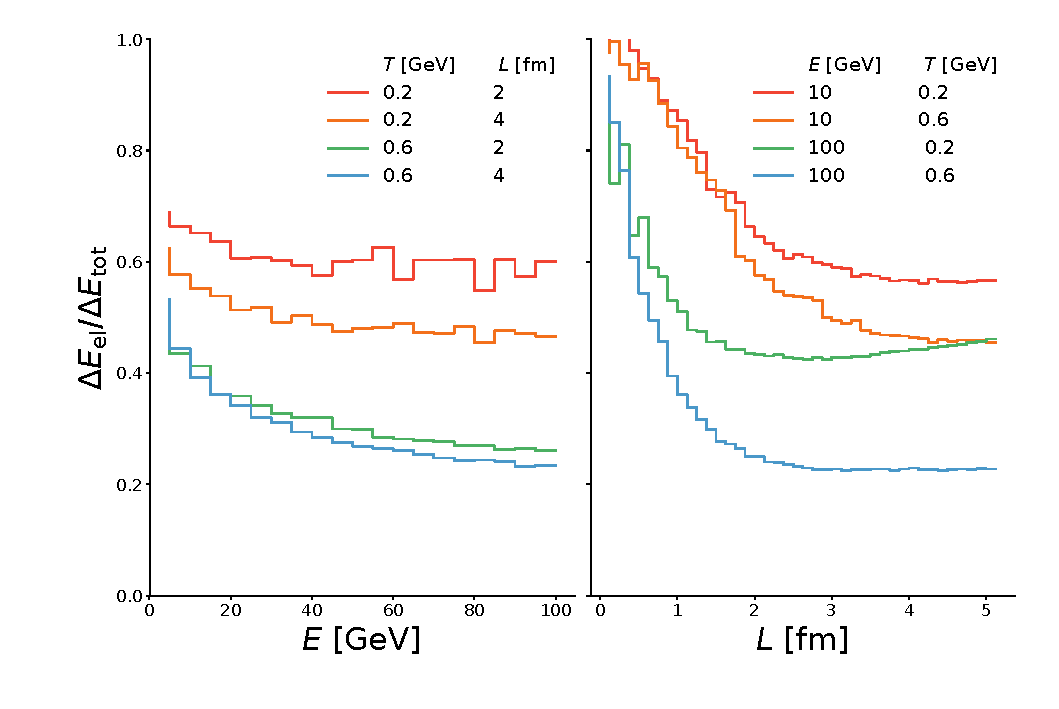
\includegraphics[width=0.85\textwidth]{fig/charm-plot/el_vs_inel.pdf}
\end{center}
\onslide<2> 
\begin{center}
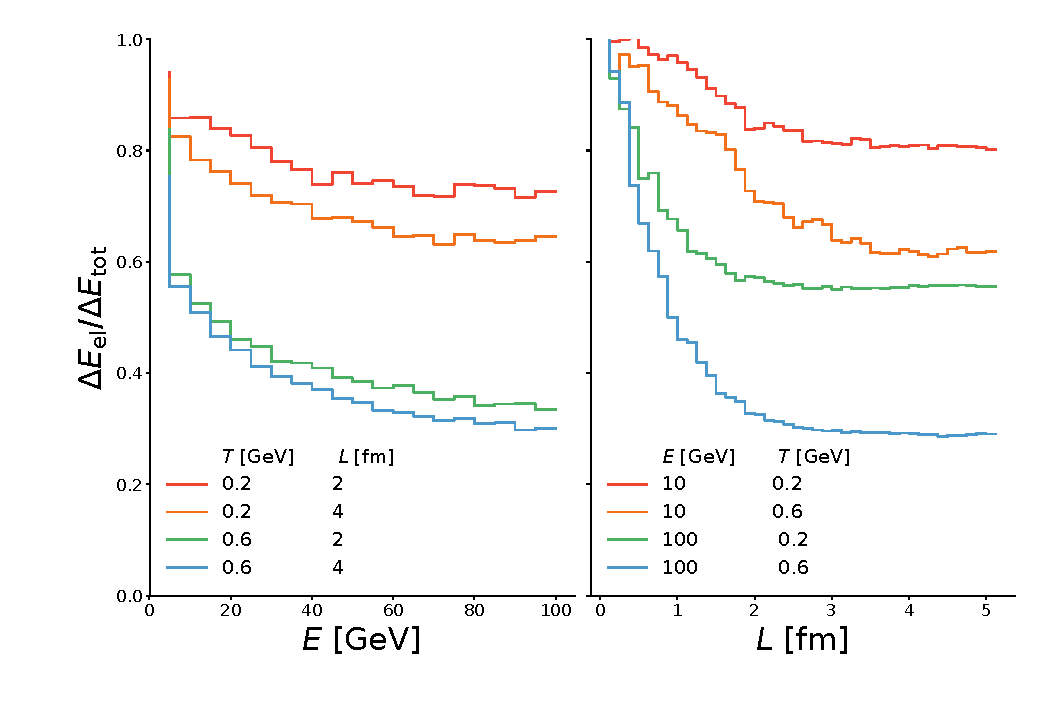
\includegraphics[width=0.85\textwidth]{fig/bottom-plot/el_vs_inel.pdf}
\end{center}
\end{overprint}
\end{frame}

\begin{frame}{pQCD: comparison of charm / bottom $R_{AA}$ in box.}

\begin{overprint}
\onslide<1> 
Something like what Shanshan compares in the HQ collaboration. Heavy quark produced according to parametrized spectra and then propagates in static box for $\Delta t = 4$ fm/c. 
\onslide<2-> 
If we use the same power law spectra $\propto p_T^{3.9}$, it appears there is less "suppression" for bottom.
\end{overprint}

\begin{overprint}
\onslide<1> 
\begin{center}
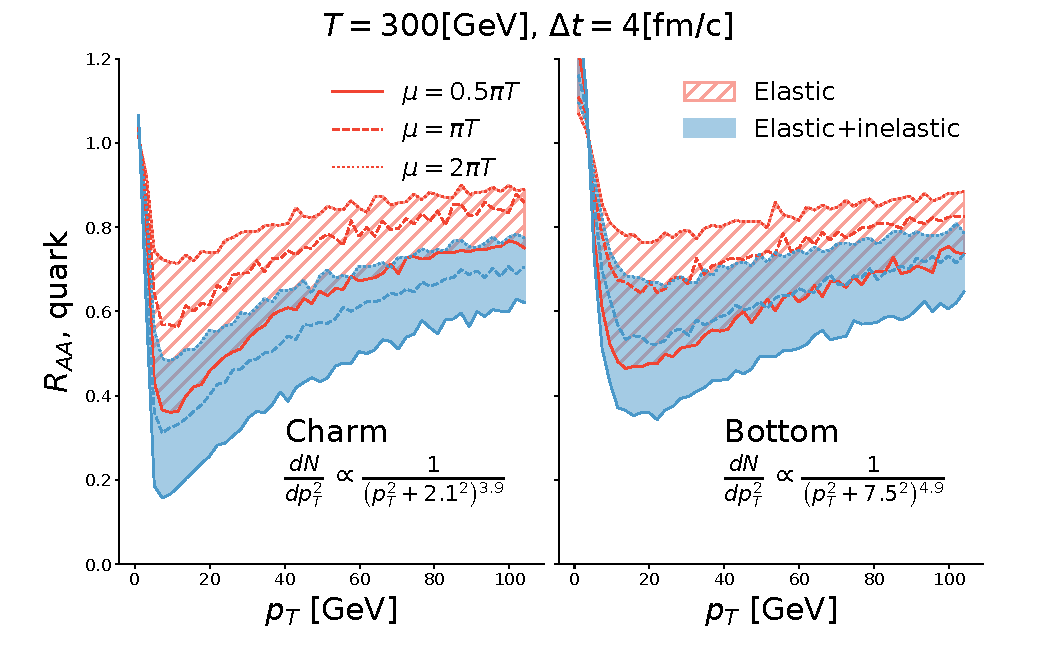
\includegraphics[width=0.9\textwidth]{fig/compare-plot/Box_Raa.pdf}
\end{center}
\onslide<2-> 
\begin{center}
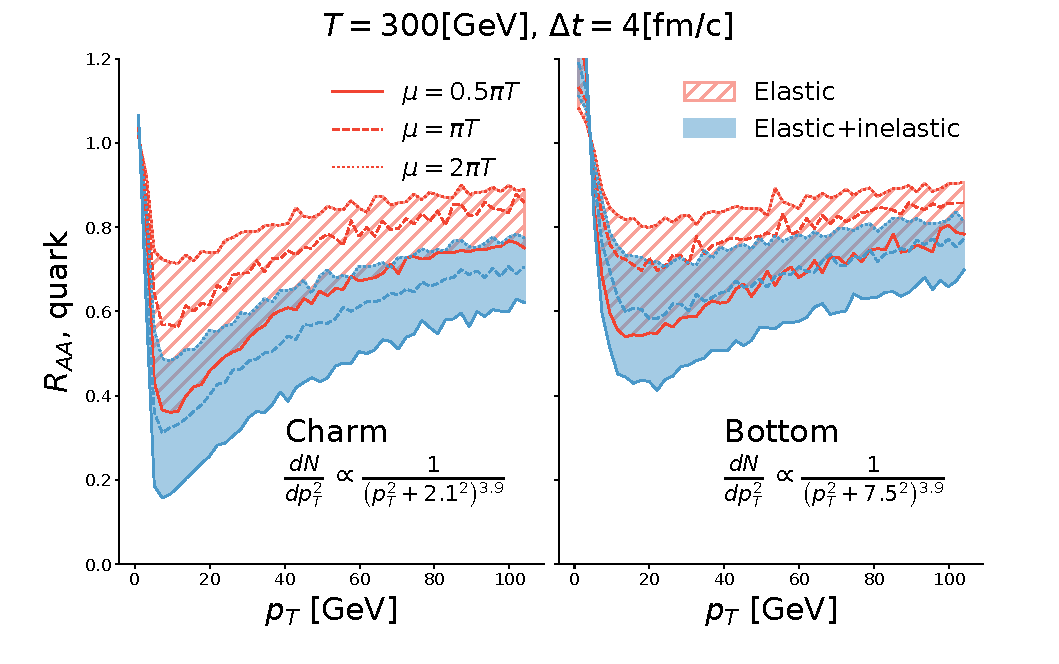
\includegraphics[width=0.9\textwidth]{fig/compare-plot/same_Box_Raa.pdf}
\end{center}
\end{overprint}

\end{frame}


\begin{frame}{Diffusion component}
Role of pQCD and diffusion,
\begin{itemize}
\item pQCD component: highly anisotropic scatterings ($\mu$).
\item Diffusion component: what is missing from pQCD ($a,b,c...$).
\begin{itemize}
\item[(1)] Non-perturbative origin.
\item[(2)] Assume to be isotropic.
\item[(3)] Assume it is pure diffusion, without induce extra radiation.
\end{itemize}
\end{itemize}
Choose a parametrization,
\begin{itemize}
\item Need mass dependence. Currently all parameters are fitted to charm meson data. But to calculate bottom quark, we probably need,
\begin{itemize}
\item[(1)] a new fit
\item[(2)] rescale it by an {\it ad hoc} mass-dependence.
\item[(3)] *start with a simple parametization with mass dependence (also based on assumptions) and fit to both charm and bottom.
\end{itemize}
\end{itemize}
\end{frame}

\begin{frame}{Diffusion: parametrization with mass (extremely na\"ive)}
For example, pQCD cross-section at small $t$ looks like,
\begin{eqnarray}
\nonumber
\frac{d\sigma}{dt} = \frac{1}{(s-M^2)^2} \frac{(s-M^2)^2}{(t-m_D^2)^2}
\end{eqnarray}
What if there are non-perturbative corrections (na\"ive guess),
\begin{eqnarray}
\nonumber
\frac{d\sigma}{dt} = \frac{1}{(s-M^2)^2} \left\{ \frac{(s-M^2)^2}{(t-m_D^2)^2}\left(1 + {\color{blue}A\frac{\Lambda^2}{-t}}\right) + {\color{red} B\frac{\Lambda^2}{\left(\sqrt{s}-{M^*}^2\right)^2+\Lambda^2}} \right\}
\end{eqnarray}
\begin{itemize}
\item {\color{blue} Blue:} maybe NP effect gives heavy quark a different form factor.
\item {\color{red} Red:} maybe NP effect allows resonances.
\end{itemize}

Eventually, they just contribute to diffusion coefficient,
\begin{eqnarray}
\nonumber
\frac{\hat{q}}{T^3} \sim  {\color{blue}a\frac{\Lambda^2}{T^2}} + {\color{red}b\frac{\Lambda^2}{ET}}
\end{eqnarray}
\end{frame}

\begin{frame}{Next:}
\begin{itemize}
\item Settled down the pQCD component (I think this part is completed).
\item Work on the Hybrid model right now. Few problems to solve
\begin{itemize}
\item A discretization scheme for the Langevin equation in the presence of scatterings.
\item Reasonable parametizations that include mass dependence.
\end{itemize}
\end{itemize}

\end{frame}

\begin{frame}{Default pQCD v.s. CMS data}
\begin{itemize}
\item pQCD sector has one parameter meidium scale $\mu_0$
\begin{eqnarray}
\nonumber
\alpha_s = \alpha_s(\max\{Q, \mu_0 \pi T \})
\end{eqnarray}
\item A linear search $-1.6 \leq \log(\mu_0) \leq 0.8, N=13$. Correspond to $0.2 \leq \mu_0 \leq 2.2$.
\item CMS data at $\sqrt{s} = 5.02$ TeV, $R_{AA}, v_{2}$, $p_T > 10 \textrm{ GeV}$, stat error only. $v_2$ errorbars are reduced by a factor $3$, because there are much less data points compared to $R_{AA}$.
\item Bulk evolution, freestreaming $\tau_0 = 0.3$ and $0.6$ [fm/c] + viscous hydro + UrQMD.
\item Nuclear PDF, nCTEQ15np and EPS09s
\end{itemize}
\end{frame}

\begin{frame}{Bulk observables}
\begin{itemize}
\item Make sure the integrated bulk observables are not sensitive to the bulk freestreaming time $\tau_0$.
\item Here, heavy quark does not interaction with medium until $\tau_0$. 
\item Varying $\tau_0$ assesses how sensitive the HQ observables are to the dynamics during $<1$ fm/c $\longrightarrow$ pre-equilibrium modeling necessary?
\end{itemize}
\begin{center}
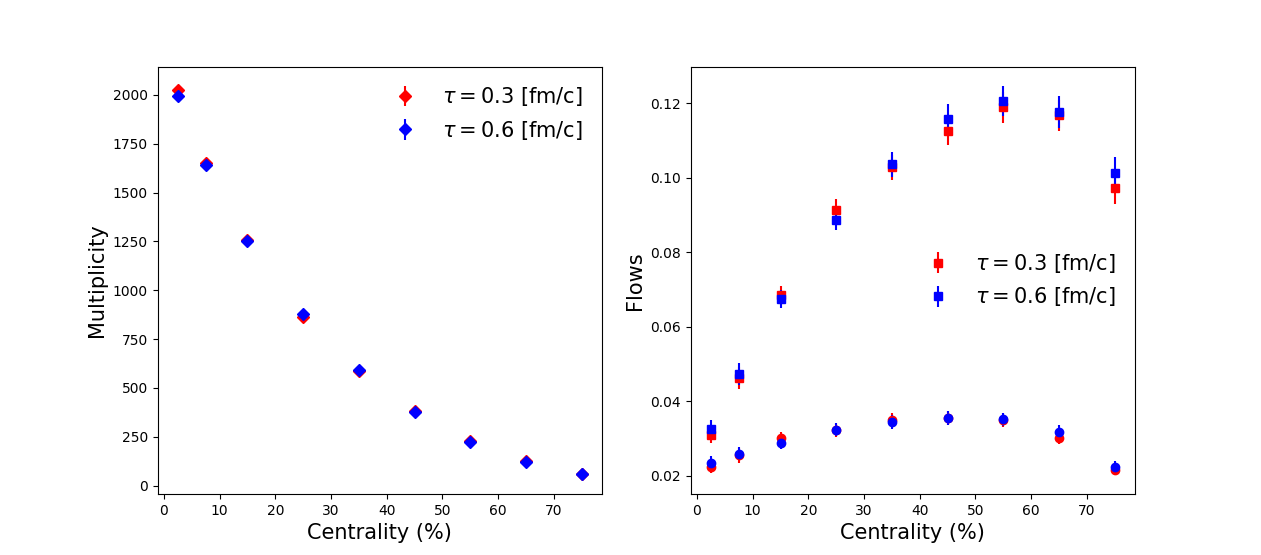
\includegraphics[width=\textwidth]{fig/mu-tune/Compare_soft.png}
\end{center}
\end{frame}

\begin{frame}{Fit quality with $\tau_0 = 0.6, 0.3$ fm/c}
\begin{overprint}
\onslide<1>
With $\tau = 0.3$ fm/c: elastic process overshoots central $R_{AA}$.
\onslide<2>
With $\tau = 0.3$ fm/c: elastic+inelastic processes fit high-$p_T$ $R_{AA}$ pretty well. Flows are still systematically underestimated.
\onslide<3>
With $\tau = 0.6$ fm/c: elastic+inelastic processes.
\end{overprint}

\begin{overprint}
\onslide<1>
\begin{center}
\includegraphics[width=\textwidth]{fig/mu-tune/{posterior-high-pT-tau=0.3-elastic}.png}
\end{center}
\onslide<2>
\begin{center}
\includegraphics[width=\textwidth]{fig/mu-tune/{posterior-high-pT-tau=0.3}.png}
\end{center}
\onslide<3>
\begin{center}
\includegraphics[width=\textwidth]{fig/mu-tune/{posterior-high-pT-tau=0.6}.png}
\end{center}
\end{overprint}

\end{frame}

\begin{frame}{Fitted $\mu$ with $\tau_0 = 0.6, 0.3$ fm/c}
\begin{overprint}
\onslide<1>
With $\tau = 0.3$ fm/c, elastic process needs a large coupling constant $\mu_0 \sim 0.37$. Decreasing $\mu$ does not always increase interaction strength due to increased screening. For example $\hat{q} \sim T^3 \alpha_s^2 \ln(1/C\alpha_s)$. The extreme is around $\mu_0 \sim 0.37$.
\onslide<2>
With $\tau = 0.3$ fm/c, elastic+inelastic process prefers $\mu_0 \sim 0.65$. \\
Usually people estimate the in-medium coupling with $\alpha_s^*(\pi T <\mu<4\pi T)$.
\onslide<3>
With $\tau = 0.6$ fm/c, pQCD needs a small $\mu_0 \sim 0.45$ to be compatible with data.
\end{overprint}

\begin{overprint}
\onslide<1>
\begin{center}
\includegraphics[width=0.58\textwidth]{fig/mu-tune/{posterior-mu-high-pT-tau=0.3-elastic}.png}
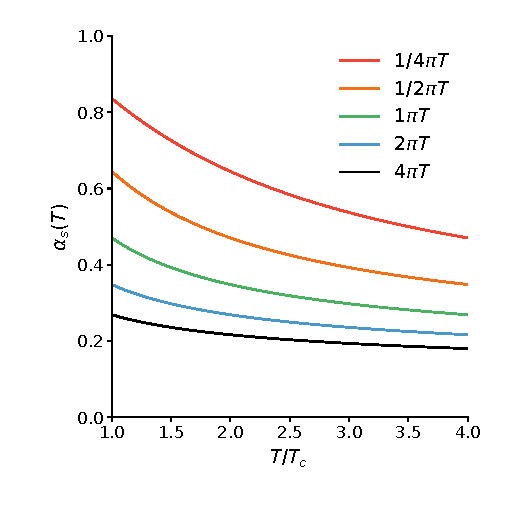
\includegraphics[width=0.42\textwidth]{fig/alpha_s_at_T.pdf}
\end{center}
\onslide<2>
\begin{center}
\includegraphics[width=0.58\textwidth]{fig/mu-tune/{posterior-mu-high-pT-tau=0.3}.png}
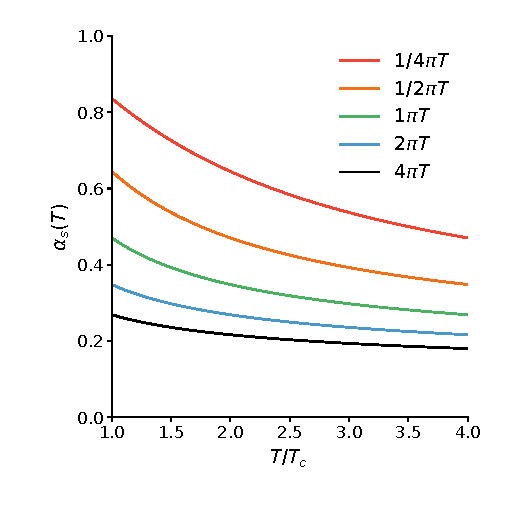
\includegraphics[width=0.42\textwidth]{fig/alpha_s_at_T.pdf}
\end{center}
\onslide<3>
\begin{center}
\includegraphics[width=0.58\textwidth]{fig/mu-tune/{posterior-mu-high-pT-tau=0.6}.png}
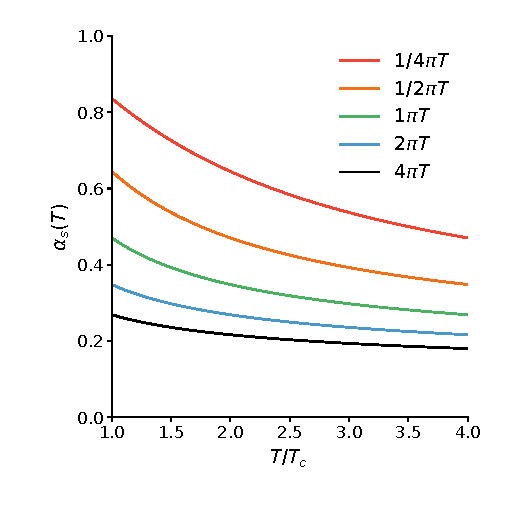
\includegraphics[width=0.42\textwidth]{fig/alpha_s_at_T.pdf}
\end{center}
\end{overprint}
\end{frame}

\begin{frame}{Summary of one-parameter fit}
\begin{itemize}
\item The $\mu_0$ parameter, unlike K-factor, cannot arbitrarily increase the strength of interaction. $\mu_0 \sim 0.37$ as a lower bound.
\item Elastic + inelastic process can fit high-$p_T$ $R_{AA}$.
\item Flows are systemically lower than data.
\item Nuclear PDF stongly affects low $p_T$ $R_{AA}$ but not flows.
\item The best value of the $\mu_0$ parameter depends (not too strong) on the time we turn on the interaction ($\tau_0=0.3, 0.6$ fm/c).
\end{itemize}

\end{frame}

\begin{frame}{For publication}
New model: hybrid approach
\begin{itemize}
\item Pure pQCD approach with the benchmark fit.
\item Pure diffusion, referring to Shanshan, Yingru's work. A well motivated parametization.
\item A calibration on hybrid model, compared to Yingru's work.
\item To answer a question on what else do we need apart from leading order pQCD interaction.
\end{itemize}

Pre-equilibrium effects, PCM, ... \\

Continue heavy flavor $R_{AA}$ in proton-lead.\\


\end{frame}


\end{document}
